\ProvidesFile{ch1.tex}[Chapter1]

\chapter{Single molecule localization microscopy}
\ix{physics//Physics appendix}

\section{Introduction}

In the quest to understand cellular function, biologists aim to directly observe the processes enabling cells to maintain homeostasis and respond dynamically to internal and environmental cues at the molecular level. Super-resolution (SR) microscopy techniques have emerged as a pathway to this aim, surpassing the classical Abbe diffraction limit of optical resolution: $\lambda/2\mathrm{NA}$ where $\lambda$ is the emission wavelength and $\mathrm{NA}$ is the numerical aperture of an objective lens. Fluorescence microscopy techniques continually push the resolution boundary towards nanometer scales, facilitating imaging of cellular structures with a level of detail previously achievable only with electron microscopy (EM). Concurrently, SR techniques retain optical microscopy advantages in biological experiments, including sample preservation, imaging flexibility, and target specificity. SR enables extraction of quantitative information on spatial distributions and often absolute numbers of proteins, nucleic acids, or other macromolecules within subcellular compartments.

Many SR methods are based on wide-field (WF), total internal reflection fluorescence (TIRF) or confocal microscope setups and fundamentally differ in how fluorescently labeled samples are excited and how the emitted photons are detected. Here, I focus on single-molecule localization microscopy (SMLM) techniques – a class of SR diffraction-unlimited SR methods which leverage fluorescence intermittency to resolve fluorophores in the sample who’s spatially overlapping point spread functions would otherwise render them unresolvable at the detector. SMLM approaches, such as direct-STORM (dSTORM) have become quite popular because they can be implemented at low cost on conventional, camera-based, wide-field setups, shifting the complexity to biological sample preparation and image post processing. Common strategies for the temporal separation of molecules involve transient intramolecular rearrangements to switch from dark to fluorescent states or the exploitation of non-emitting molecular radicals. For example, in dSTORM, rhodamine derivatives can undergo intersystem crossing to a triplet state, which can be reduced by thiols to form a dark radical species. The dark state can then be quenched by oxidative processes, driving the fluorophore back to its ground state. 

In SMLM applications, we seek the position and intensity of isolated fluorophores as well as to estimate the accuracy and precision of these parameters. Accuracy is a measure of the systematic error or bias, and precision is a measure of the statistical error of an estimator. To generate super-resolution images using SMLM, single emitters are located, and using the mosaic of their found positions, we produce a kernel density estimate (KDE). Such KDEs are often Gaussian, and are used to generate the final super-resolution images. The width of one such placed Gaussian function, $\sigma$ is given by the precision of the fluorophore position localization. Therefore, in SMLM, it is necessary to both find the parameters and estimate their precision. Reported values are in the range of 20–70 nanometers. In the following section, we derive a fundamental statistical description of fluorophore detection in SMLM, which is compatible with a coherent state of the quantized electromagnetic field. This description is necessarily simplified - background rates of light detection may vary across the field of view, and the fluorophore emission rate of chemically identical fluorophores can vary owing to effects such as uneven illumination profile, dipole orientation or different optical path lengths.

\subsection{Elementary mathematical theory of SMLM}


\begin{equation}
\omega = i_{0}\int O(u)du\int O(v)dv
\end{equation}

where $i_{0} = \eta N_{0}\Delta$. The optical impulse response $O(u,v)$ is often approximated as a 2D isotropic Gaussian with standard deviation $\sigma$ (Zhang 2007). The parameter $\eta$ is the photon detection probability of the sensor and $\Delta$ is the exposure time. $N_{0}$ represents the number of photons emitted.

Using the common definition $\mathrm{erf}(z) = \frac{2}{\sqrt{\pi}}\int_{0}^{t}e^{-t^{2}}dt$,

\begin{equation}
\int O(u)du = \frac{1}{2}\left(\mathrm{erf}\left(\frac{u_{k}+\frac{1}{2}-u_{0}}{\sqrt{2}\sigma}\right) -\mathrm{erf}\left(\frac{u_{k}-\frac{1}{2}-u_{0}}{\sqrt{2}\sigma}\right)\right)
\end{equation}

For the sake of generality, the number of photoelectrons at a pixel $k$, $\bold{s}_k$, is  multiplied by a gain factor $g_k \;[\mathrm{ADU}/e^{-}]$, which is often unity. The readout noise per pixel $\zeta_{k}$ can be Gaussian with some pixel-specific offset $o_{k}$ and variance $\sigma_{k}^{2}$. Ultimately, we have a Poisson component of the signal, which scales with $N_{0}$ and may have Gaussian component, which does not. Therefore, in a single exposure, we measure: 

\begin{equation}
\bold{x}_t = \bold{s}_t + \bold{\zeta}
\end{equation}

What we are after is the likelihood $p(\bold{x}_{t}\lvert\theta)$ where $\theta$ are the molecular coordinates. Fundamental probability theory states that the distribution of $\bold{x}_{k}$ is the convolution of the distributions of $\bold{s}_{k}$ and $\zeta_{k}$,

\begin{equation}
p(\bold{x}_{t}\lvert\theta) = A\sum_{q=0}^{\infty} \frac{1}{q!}e^{-\omega_{k}}\omega_{k}^{q}\frac{1}{\sqrt{2\pi}\sigma_{k}}e^{-\frac{(\bold{x}_{k}-g_{k}q-o_{k})}{2\sigma_{k}^{2}}}
\end{equation}

where $P(\zeta_{k}) = \mathcal{N}(o_{k},\sigma_{k}^{2})$ and $P(S_{k}) = \mathrm{Poisson}(g_{k}\omega_{k})$,  $A$ is some normalization constant. In practice, (4) is difficult to work with, so we look for an approximation. We will use a Poisson-Normal approximation for simplification. Consider,

\begin{equation}
\zeta_{k} - o_{k} + \sigma_{k}^{2} \sim \mathcal{N}(\sigma_{k}^{2},\sigma_{k}^{2}) \approx \mathrm{Poisson}(\sigma_{k}^{2})
\end{equation}

Since $\bold{x}_{k} = \bold{s}_{k} + \zeta_{k}$, we transform $\bold{x}_{k}' = \bold{x}_{k} - o_{k} + \sigma_{k}^{2}$, which is distributed according to 

\begin{equation}
\bold{x}_{k}' \sim \mathrm{Poisson}(\omega_{k}')
\end{equation}

where $\omega_{k}' = g_{k}\omega_{k} + \sigma_{k}^{2}$. This result can be seen from the fact the the convolution of two Poisson distributions is also Poisson. The quality of this approximation will degrade with decreasing signal level, since the Poisson distribution does not retain its Gaussian shape at low expected counts. Nevertheless, the quality of the approximation can be predicted by the Komogonov distance between the convolution distribution (4).

\begin{figure}
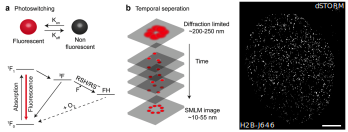
\includegraphics[width=\textwidth]{figures/Intro.png}
\caption{\textbf{Stochastic optical reconstruction microscopy (STORM)}. (A) Single molecules are resolved by separating their fluorescent emission in time, using fluorophores with multiple photophysical states (B) Example super-resolution image of H2B protein in a living Hela cell nucleus at 37C, 5 percent CO2. Image reconstructed from $10^{3}$ 10ms frames. Scalebar 5um.}
\end{figure}

\clearpage
\begin{figure}
\begin{center}
\includegraphics[width=16cm]{figures/Noise.png}
\end{center}
\caption{\textbf{Noise model for CMOS cameras used for MLE}. (left)) CMOS offset for zero incident photons (middle) CMOS variance for zero incident photons (upper right) Cumulative mass function for the convolution distribution and its Poisson approximation for rate parameter $\mu_{k} = 500$ counts (lower right) Komogonov distance measured as a function of rate parameter $\mu_{k}$}
\end{figure}


\subsection{The definition of resolution in SMLM}

The distribution of a particular biomolecule in the cell can be described as a probability density over a two-dimensional space, casting super-resolution as a density estimation problem. Intuitively, the spatial resolution of SMLM images then increases as we draw more samples from this density - a concept which is made mathematically precise by the so-called Fourier ring correlation or FRC. Using FRC, one can compute image resolution as the spatial frequency at which a correlation function in the frequency domain drops below a threshold, typically taken to be $1/7$ (See Supplement). According to this theory, reducing localization uncertainty while increasing the number of samples, results in an increase in image resolution (Nieuwenhuizen 2013). However, there remains a fundamental limit to the the minimal localization uncertainty which can be obtained.


\begin{figure}
\begin{center}
\includegraphics[width=16cm]{figures/MCMC.png}
\end{center}
\caption{\textbf{Computing epistemic uncertanties with Metropolis-Hastings}. (top left) Simulated point spread function for $N_{0}=10^{3}$ photons with a red x at $x_{\mathrm{MLE}}$ and $y_{\mathrm{MLE}}$ (bottom left) Acceptance rate of Markov chain (middle) Markov chains sampling from the posterior distribution on molecule coordinates in 3D, with the maximum likelihood estimation in dashed blue (right) Estimated posterior marginals on the localization parameters with their respective uncertanties}
\end{figure}


\begin{equation*}
\mathrm{FRC}(q) = \frac{\sum_{\vec{q}\in\mathrm{circle}}\tilde{f_{1}}(\vec{q})\tilde{f_{2}}(\vec{q})^{*}}{\sqrt{\sum_{\vec{q}\in\mathrm{circle}}\lvert f_{1}(\vec{q})\lvert^{2}}\sqrt{\sum_{\vec{q}\in\mathrm{circle}}\lvert f_{2}}(\vec{q})\lvert^{2}}
\end{equation*}


Localization uncertainty, typically the RMSE of a maximum likelihood or similar statistical estimator, is bounded from below by the inverse of the Fisher information matrix, known as the Cramer-Rao lower bound (Chao 2016). Localization uncertainties in sparse conditions are often tens of nanometers, although recent work on integration of Bayesian priors with modulation enhanced SMLM (meSMLM) or structured illumination with MINFLUX, has reduced spatial resolution below to a few nanometers (Kalisvaart 2022, Gwosh 2020). Nevertheless, managing the increase in localization uncertainty at high labeling density remains a major bottleneck to SMLM. Static uncertainty due to molecular crowding can be partially amelioriated by using pairwise or higher-order temporal correlations within a pixel neighborhood, known as stochastic optical fluctuation imaging or SOFI (Dertinger 2009). Other approaches such as stimulated emission and depletion (STED) imaging bring control over the photophysical state of a chosen subset of the sample, yet the need for laser scanning prevents widespread application in live-cell studies. The spatial resolution and relative simplicity of SMLM techniques remains unmatched, inciting an effort to increase the resolution of SMLM techniques and explore avenues towards time resolved SMLM.

\clearpage
\begin{figure}
\begin{center}
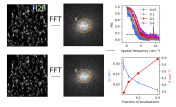
\includegraphics[width=16cm]{figures/FRC.png}
\end{center}
\caption{\textbf{Noise model for CMOS cameras used for MLE}. (left)) CMOS offset for zero incident photons (middle) CMOS variance for zero incident photons (upper right) Cumulative mass function for the convolution distribution and its Poisson approximation for rate parameter $\mu_{k} = 500$ counts (lower right) Komogonov distance measured as a function of rate parameter $\mu_{k}$}
\end{figure}



\subsection{The Cramer-Rao lower bound}

The Poisson approximation is also convenient for computing the Fisher information matrix for $\theta_{\mathrm{MLE}}$ and thus the Cramer-Rao lower bound, which bounds the variance of a statistical estimator of $\theta_{\mathrm{MLE}}$, from below (Chao 2016). The Fisher information is

\begin{equation}
I_{ij}(\theta) = \underset{\theta}{\mathbb{E}}\left(\frac{\partial \ell}{\partial\theta_{i}}\frac{\partial\ell}{\partial\theta_{j}}\right) 
\end{equation}

Let $\mu_{k}' = g_{k}\mu_{k} + \sigma_{k}^{2}$. For an arbitrary parameter,

\begin{align*}
\frac{\partial \ell}{\partial \theta_{i}} &= \frac{\partial}{\partial \theta_{i}} \sum_{k}  x_{k}\log x_{k} + \mu_{k}' - x_{k}\log\left(\mu_{k}'\right)\\
&= \sum_{k} \frac{\partial \mu_{k}'}{\partial\theta_{i}} \left(\frac{\mu_{k}'-x_{k}}{\mu_{k}'}\right)
\end{align*}

\begin{equation*}
I_{ij}(\theta) = \underset{\theta}{\mathbb{E}}\left(\sum_{k}\frac{\partial \mu_{k}'}{\partial\theta_{i}}\frac{\partial \mu_{k}'}{\partial\theta_{j}} \left(\frac{\mu_{k}'-x_{k}}{\mu_{k}'}\right)^{2}\right) = \sum_{k}\frac{1}{\mu_{k}'}\frac{\partial \mu_{k}'}{\partial\theta_{i}}\frac{\partial \mu_{k}'}{\partial\theta_{j}}
\end{equation*}



